\chapter{\label{c:speedmeter-intro}The \SSMEXPT{}: introduction and infrastructure}

\section{Concept}
\begin{itemize}
  \item Usual literature review: use 2nd year report, Living Review, Graef et al, etc...
  \item Show Michelson response and noise. This should be radiation pressure dominated below the pole. Relate this to the analytical response equation I used in the controls paper for a Michelson.
  \item Introduce Sagnac speedmeter, showing it has better quantum noise IN ABSENCE OF ASYMMETRIES, and thus better overall sensitivity for equivalent shot noise. DON'T SHOW THE SSM SENSITIVITY HERE.
  \item Use Stefan D's labbook entry for response functions: p5648
  \item Introduce losses to show the degrading effect they have, introducing ``Michelson-like'' sensitivity. The main thing to show here is the effect on the quantum noise when there are asymmetries, like test mass asymmetry. This broadens the peak around the suspension resonance, which introduces the Michelson-like sensitivity.
  \item Mention significance of M8/M9/M10's reflectivity (c.f. loss) which can be expanded later in the controls chapter.
\end{itemize}

As discussed in Section\,\ref{sec:sql}, the \gls{SQL} limits the sensitivity of classical interferometers. Arising from the Heisenberg Uncertainty Principle, the quantum noise present within a classical interferometer\footnote{Note the misnomer: a \emph{classical} interferometer can still be limited by \emph{quantum} noise. The name refers to the readout technique, namely the measurement of classical light power to determine displacement.} It has been known since the time of John von Neumann \note{CITE!} that the use of certain observables can avoid the limit set by the uncertainty principle.

In 1990, Braginsky and Khalili showed that the measurement of momentum, known to be a \emph{quantum non-demolition} (\gls{QND}) observable, offers the ability to surpass the \gls{SQL} in interferometric measurement \cite{Braginsky1990}.

\subsection{Measurement of speed}


\section{Implementation}

Some technical challenges in the implementation of the speedmeter are discussed in this chapter. Certain topics involve substantially more scientific endeavour and are thus presented as discrete chapters: the control of the primary degree of freedom of the speedmeter, presented in Chapter X; and a proof-of-principle experiment to demonstrate a new type of actuator, presented in Chapter Y.

\subsection{Experimental design}
\note{Discuss the experiment layout, power, cavity lengths, etc. Introduce the real sensitivity curves here.}

\subsection{Mechanics}
\note{Vacuum system requirements, tanks, optical table, suspensions, seismic noise, etc.}

\subsection{Layout}

\begin{figure}
  \centering
  \includegraphics[width=\columnwidth]{graphics/generated/from-svg/40-speedmeter-layout.pdf}
  \caption{\label{fig:ssm-layout}\SSMEXPT{} layout.}
\end{figure}

\subsection{Sensing and control}

\subsubsection{Avoidance of ground loops}

One of the main issues faced by experiments involving numerous interfaces between digital and analogue devices is the creation of ground loops. Effectively an antenna.

\note{Avoidance of ground loops, interfacing with CDS, in-vacuum wiring: why it needs careful thought, etc}
\note{Display wiring diagrams in landscape mode, full page}

\note{Generate A4 versions of wiring diagrams for inclusion here.}

\subsubsection{Connectors}
\note{How we avoided plugging the wrong things in, i.e. why we use DB9/DB15/DB25 etc.}
\note{Differential sending - take stuff from HV chapter on CMRR?}

\subsubsection{In-vacuum signalling}
\note{Octopus cables, strain relief housing, etc.}

\begin{figure}
  \centering
  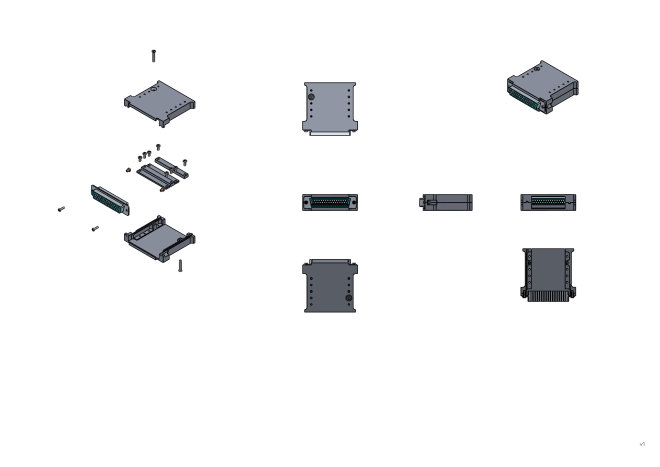
\includegraphics[width=0.75\columnwidth]{graphics/40-db50-housing.png}
  \caption{In-vacuum DB50 housing for octopus cable.}
  \label{fig:db50-housing}
\end{figure}

\subsubsection{Auxiliary coil drivers}
\note{Put aux coil driver stuff here}
\note{Auxiliary coil driver subrack wiring design / motivation / assembly}
\note{Backplane board design - talk about rationale, show Eagle diagrams, etc.}